\documentclass[11pt,twoside]{article}
\usepackage[a4paper,
            left=30mm,
            right=15mm,
            top=15mm,
            bottom=20mm]{geometry}
\usepackage{enumerate}
\usepackage{latexsym,booktabs}
\usepackage{amsmath,amssymb}
\usepackage{algpseudocode}
\usepackage{algorithm}
\usepackage{graphicx}
\usepackage{subcaption}
\usepackage{float}
\usepackage{multirow}
\usepackage[table,xcdraw]{xcolor}
\usepackage[singlespacing]{setspace}

\geometry{a4paper,left=3cm,right=2.0cm, top=2cm, bottom=2.0cm}

\newtheorem{Definition}{Definition}
\newtheorem{Theorem}{Theorem}
\newtheorem{Lemma}{Lemma}
\newtheorem{Algorithm}{Algorithm}
\numberwithin{Theorem}{section}
\numberwithin{Definition}{section}
\numberwithin{Lemma}{section}
\numberwithin{Algorithm}{section}
\numberwithin{equation}{section}

\graphicspath{ {./images/}{./} }

\begin{document}

\pagestyle{empty}

% =============================================================================
% Title page
% =============================================================================
\begin{titlepage}
\vspace*{.5em}
\center
\textbf{\large{The School of Mathematics\\}}
\vspace*{1em}
\begin{figure}[!h]
\centering

\includegraphics[width=180pt]{CentredLogoCMYK.jpg}
\end{figure}
\vspace{2em}
\textbf{\Huge{Agent-based models in Vega-market-sim environment: Competing or Collusion }}\\[2em]
\textbf{\LARGE{by}}\\
\vspace{2em}
\textbf{\LARGE{Fanggang Yan}}\\
\vspace{6.5em}
\Large{Dissertation Presented for the Degree of\\
MSc in Financial Mathematics}\\
\vspace{6.5em}
\Large{August 2023}\\
\vspace{3em}
\Large{Supervised by\\Dr Jiajia Cui and Dr David Siska}
\vfill
\end{titlepage}

\cleardoublepage


\begin{center}
\Large{Abstract}
\end{center}

This paper introduces the mathematical foundation of reinforcement learning and proposes three algorithms (DQN, AC, and CAC) for training automated traders in the futures market on Vega’s platform. The CAC model demonstrates superior performance and is chosen for in-depth numerical experimentation. Four traders are categorized into three parties: a colluding cartel, a similarly intelligent trader, and a less-informed novice trader. Results highlight that intelligent traders, especially those in collusion, exhibit significant profitability, showcasing their dominance in the market. However, while the cartel presents some resilience, the CAC model's overall robustness is found lacking during sensitivity tests, with pronounced vulnerabilities to market changes. Recommendations suggest a more comprehensive training process, robustness refinement, and varied scenario testing to improve the model’s efficacy and understanding. The study also paves the way for investigating the impact of a completely competitive market to measure the true extent of excessive profits due to collusion.
\\ \\
Keywords: Reinforcement learning, Automated traders, Futures market, Vega Protocol, Collusion, Competitive market.

\clearpage

\begin{center}
\Large{Acknowledgments}
\end{center}

First of all, I would like to say thanks to my supervisors, Jiajia Cui and David Siska. Their rigorous and supervision and cordial welcome have made this research prosper. They renewed my outlook on academic supervision: it is about an afternoon of meticulousness revolving around a thought-provoking topic, but in the meantime, it is also, even more importantly, a cup of coffee that broke the ice between heart and heart, a kind gesture from a homemade bakery and an unexpected but unforgettable peer social.

Thanks to this wondrous fleeting year, the evanescence of which reminds me to cherish every split second of the time with the people I love. Thanks to the light and scent permeating every nook and cranny of Edinburgh, which constitute my vivid yet soon-to-be nostalgic collage of invaluable memories. Thanks to the caprice of the weather, a constant caveat to a mathematics student that every prediction has its confidence interval. We are to model but not eradicate the volatility of every entity. Thanks to the eternal sunlight over summer, which has nurtured and rescued a diehard night owl from the decadence of converting to an entire vampire. 

This section is dedicated to Sherry, whose name happens to be a fine type of intense wine, which she is not cut for savouring for the sake of a missing enzyme, unfortunately.  I am immensely beholden to nothing but her existence, which functions as an inexhaustible source of my assurance.

Thanks to The Guys. I know it’s somehow a euphemism, but jotting down the original version might send me to a bunch of official hearings and fail this degree. Inclusivity and diversity are the prevailing themes in this group. We are from everywhere and tailored into disparate personalities: a gasbag with endless whimsical topics, a paragon with no flaw to the best of my knowledge, a mischievously mature man with a thousand cracking-you-up jokes, and the nobody who is me. The most incredible serendipity of mine over this year is that I have, by the merest chance, become friends with you all. 

Thanks to JAK, a nickname of novelty for a group of friends of mine (credit to one of The Guys). The extensive range of topic on our table completes what I am in shortage of as a former science and mathematics student. Every night in the future when i try to recollect the bits of my memory, I am more than certain that the time with you guys chitchatting in every decent pub of Edinburgh will be scintillating indelibly.  

Last “and the least”, thank you to those who actually have proceeded to this very ending of the long-winded yet insignificant part. This running-over acknowledgement will have been the reminiscences that remind me of this year of surreal adventures. I appreciate your patience and the trees that might sadly demise every time this extra page is printed.

\clearpage

\begin{center}
\Large{Own Work Declaration}
\end{center}

\noindent I confirm that all this work is my own except where indicated, and that I have:
\begin{itemize}
    \item clearly referenced/listed all sources as appropriate;
    \item referenced and put in inverted commas all quoted text (from books, web, etc);
    \item given the sources of all pictures, data etc. that are not my own;
    \item not made any use of the report(s) or essay(s) of any other student(s) either past or present;
    \item not sought or used the help of any external professional academic agencies for the work;
    \item acknowledged in appropriate places any help that I have received from others (e.g. fellow students, technicians, statisticians, external sources);
    \item complied with any other plagiarism criteria specified in the Course handbook.
\end{itemize}
I understand that any false claim for this work will be penalised in accordance with the University regulations.
\cleardoublepage



% =============================================================================
% Table of contents, tables, and pictures (if applicable)
% =============================================================================
\pagestyle{plain}
\setcounter{page}{1}
\pagenumbering{Roman}

\tableofcontents
\clearpage
\listoftables
\listoffigures
\cleardoublepage

\pagenumbering{arabic}
\setcounter{page}{1}

\nocite{*}
\bibliographystyle{abbrv}
\clearpage

\section{Introduction}
\label{sec.intro}

As trading actively operates at the heart of the economy, futures markets have established their pivotal role across all businesses, with 29.32 billion contracts traded worldwide in 2022. They enable traders to buy and sell assets at a price agreed upon today, while the actual transaction is scheduled for a predetermined date in the future. This form of trading offers opportunities for speculation, hedging against price changes, and acquiring or delivering assets in the future. One of the trailblazers in this industry is Vega Protocol, a company that this paper collaborates with and is supervised by. It has developed a fully decentralised derivatives trading network, which the work of this paper is set in. Leveraging this cooperation grants us the access of real-market trading data as well as a test bed to examine the validity of the theories we propose.

Amongst all components of a futures market, market-making strategies are of central concern. Availing themselves with these strategies, market makers seek profits by placing orders, thereby facilitating the liquidity and steadiness of the market. In the context of futures markets, a market maker places their bid and quote without knowledge of competing offers, and then receives their spread once the price competition terminates. This scenario involves an intricate trade-off between the potential for higher profits and an increased probability of the order being agreed. Thus, the selection of a favourable strategy is rather delicate, further complicated by the uncertainty rooted in the behaviours of competitors.

The complexity and necessity to optimise market-making strategies has steered attention to Reinforcement Learning (RL), a subfield of Artificial Intelligence (AI) providing an efficient tool to learn from available information and make informed decisions on these strategies. RL utilises an array of agents, each learning from their interactions with the environment and other agents. In light of some branches of RL, it is possible to train agents in a model-free manner, namely, without the specification of transitions within the system. This obviates the difficulty to model an intricate system with mathematical rigour, illuminating an approach to develop favourable strategies based on solely interactions.

In the market, market makers can collude to profit from the information asymmetry, penalising those unaware of the cartel's decisions on their bids and quotes. Moreover, even without explicit information exchange, the agents hinging on the same RL algorithm and historical data tend to provide similar tenders, which might result in implicit collusive behaviours. This dissertation, "Dynamics of Market Making Algorithms in Vega-market-sim Environment: Competing or Collusion," is dedicated to utilise these aforementioned breakthroughs to investigate the impact of competition and collusion among market makers within the Vega protocol environment. To specify, this paper aims to delve into the profitability of each party and the overall welfare within the market, under the following three scenarios: 
\begin{itemize}
    \item (Competition) Each agent receives no information from others before the deal has been made;    
    \item (Explicit Collusion) There exists a cartel within which every member discloses their tender beforehand;
    \item (Implicit Collusion) A cluster of agents rely on the same RL algorithm, but no explicit information exchange occurs.
\end{itemize}

The dissertation will proceed as follows:
\begin{enumerate}
\item An extensive literature review on futures markets, market making, and Reinforcement Learning.
\item A concise introduction to the Vega Protocol environment with a focus on its underlying mechanisms.
\item Mathematical modelling and interpretation of the problem at hand.
\item Explanation of the algorithmic methodology employed in this research.
\item Presentation of the numerical results pertaining to the problems under consideration.
\item Analysis and discussion of the project's outcomes.
\item A summary of the key findings and suggestions for future research.
\end{enumerate}

%Particularly Section \ref{sec:background} is good!
\clearpage

\section{Background}
\label{sec:background}
The objective of this section is to provide essential background that underlies this article, obviating potential barriers for readers to understand without additional references.
\begin{itemize}
\item To begin with, the futures market, in which our problem is set, is introduced, including its history, significance, dynamic, strength and complexity. 
\item With the established comprehension of the market dynamics, the theories and techniques about Stochastic Control (SC) are explained, equipping us with the tools to model and address the problem from a mathematical perspective. 
\item As a transition from theory to computational application, the Reinforcement Learning (RL) is highlighted with its theoretical association to SC problems and its practical aspect mentioned.
\end{itemize}

\clearpage

\subsection{Futures Market}
\label{sec:Market}
Derivatives have accrued its [their] preponderance in the financial sector since 1848, the year when the inception of the Chicago Board of Trade (CBOT) unfurled the blueprint of a derivatives exchange. The CBOT was initiated with the mission to standardise and stabilise the quantities and qualities of grain trades. However, its innovative reach transcended far beyond this original purpose, with the establishment of its financial infrastructure and the incorporation of an extensive variety of assets, such as commodities, currencies, equities, and bonds. It was not many years later when the first future-type contract was developed throughout the evolution [in the evolution process]. This is the prototype and genesis of the burgeoning and prospering \emph{futures market}, the centrepiece of this subsection's discussion.

The primary financial instrument traded in a futures market is \emph{futures contracts}, an agreement to trade an asset at a designated time for a predetermined price. A future contract involves the buyer and the seller, two parties that do not necessarily have a direct connection with each other. Thus, there arises the requirement of an intermediary institution to facilitate, oversee, and regulate such a contract. In the context of the futures market, this intermediary is referred to as an \emph{exchange}.\cite{market}

An exchange is obliged to determine the features and specifics of each futures contract, which includes but is not limited to the following aspects:
\begin{itemize}
\item \emph{Underlying asset}: Stripped of its complexity, a futures contract is, after all, a trade pertaining to a certain type of asset, be it commodities or financial assets. Consequently, the underlying asset is of vitality in contract selection, price evolution, and risk evaluation, and therefore of critical consideration for both parties and their exchange. For commodity futures contracts, the exchange has to stipulate the grade(s) that the delivered goods should meet, thereby ensuring and supervising the quality of the commodities involved; however, for contracts underpinned by financial assets, the details of it [are] concrete with the clarification of the asset per se.
\item \emph{Contract size}: Contract size specifies the quantity of the asset to be delivered upon maturity. It denotes the scale of the transaction, which is also a key feature for all parties. A smaller scale implies reduced risk and illiquidity, while increases [it increases] the ratio of cost due to the commission charged by the exchange.
\item \emph{Delivery arrangement}: The time and place of the delivery are enunciated in the delivery arrangement. The exchange provides the span of time within a month when the delivery can take place, and a final date before which the delivery process should terminate. In regard to the place, it concerns those contracts involving a considerable transportation cost: if the delivery place is far from where the party with the short position plan to place their commodities, they may seek a discounted price to offset the cost needed in transportation.
\item \emph{Price quote}: The price quote defines the currency, precision, and format in which the prices will be quoted. It concretises the quote into a certain currency and discretises the price from its continuous real number form to an admissible format.
\item \emph{Price limits}: Price limits regulate the maximal fluctuation in a contract's price, conventionally on a daily basis. When the price varies beyond the permitted range within a day given by the limits, the trading is halted and does not resume until the following day. The presence of price limits aids to mitigate the excessive volatility of the market, promoting a more stable trading environment.
\item \emph{Position limits}: Position limits stipulate the range of contracts a trader can possess, precluding extreme long or short positions. The implement [implementation] of position limits bolsters the credibility of traders, discourages market manipulation, and contains potential oligarchies.
\item \emph{Trading hours}: The exchange sets the specific hours during which the futures contract can be traded.
\end{itemize}

In addition to finalising the aforementioned specifications of contracts, an exchange also undertakes the responsibility of risk management. A default occurs when one of the parties withdraws from the agreement, either due to a change in their intentions or because they have depleted the resources they were obligated to provide under the contract. Therefore, a contract without any collateral or deposit entails significant risks, which has motivated exchanges to devise the concept of \emph{margin accounts}. The two key elements of a margin account are \emph{initial margin} and \emph{maintenance margin}. 

An initial margin is the amount of capital that a trader have to deposit in their margin account upon the placement of their order. Namely, it is the deposit that grant a trader the entry to the position they are seeking. The initial margin requirement varies but ranges from 3\% to 12\% in common practice. Upon a settled initial margin, a \emph{maintenance margin}, normally 50\% to 75\% of the initial margin, is established as a threshold. Once the balance in a trader's margin account goes down to the maintenance margin, the trader receives a margin call and is obliged to replenish their account to the initial margin requirement (not maintenance margin) by the end of the next day. If one fails to top up their account, the position will be closed out. 

The balance in a margin account is also adapted to the market price, which is settled on a daily basis. At the end of each trading day, the balance of a margin account is applied with an increase equal to the investor's gain (or an deduction equal to their loss). This practice is named \emph{daily settlement} or \emph{marking to market}. Daily settlement reflects the performance of an investor's asset into their margin account, thought the limit of which the exchange oversee and regulate the risk of such a trade.

As can be seen from the mechanism of futures tradings, venturing into futures comes with benefits. By including futures in an investment portfolio, investors can access asset classes that may not be readily available in traditional markets such as stocks, bonds, and options. For those with an appetite for speculation, futures trading offers the potential for significant gains (or losses) at a faster pace compared to other markets. Companies utilize futures contracts to mitigate the risk of sudden price fluctuations. This approach is particularly advantageous for those needing to manage input prices for their products, as futures contracts allow them to lock in current prices and safeguard profits. Certain futures trades qualify for preferential tax treatment under the 60/40 rule, where 60\% of profits receive long-term capital gains treatment, and the remaining 40\% are treated as short-term capital gains. This unique structure sets futures apart from traditional stock trading in terms of tax advantages. Futures provide a more favorable margin requirement for short selling compared to stocks. Investors can risk less of their available cash for short selling positions in futures, making it an attractive option for profiting from downward market movements. However, these advantages also engender an increased risk in this market. Aside from the higher complexity which requires comprehension and proficiency in finance to address, a appreciable rate of leverage and its highly speculative involve the possibility of a significant loss, potentially greater than one's initial investment.

\clearpage

\subsection{Stochastic Control}
\label{sec:SC}
Underpinned by the futures market, tradings involving futures inherit the properties of the futures market. By their intrinsic value, tradings under this setting is an optimisation problem with stochasticity subject to certain constraints. To elucidate, the objective of each trader is to maximise their profit, and simultaneously, to evade the penalty arising from the occurrence of a closeout. However, the financial resource that an agent can leverage is circumscribed by the requirement of their margin account, leading to the constraints imposed on each trader. Meanwhile, there is randomness originated from such a mechanism— the price evolves with randomness, which presumably follows a certain stochastic process, and every transaction on the market, especially those of considerable amount, has an impact on the price, incorporating a behavioural factor. All these features guide us to seek a solution from the theorems of Stochastic Control (SC).

Stochastic control is a fundamental and sophisticated branch of applied mathematics and control theory, specifically designed to address decision-making in the presence of uncertainty and randomness. This powerful framework tackles problems where the evolution of a system is influenced not only by the decisions made by a controller but also by stochastic processes or random disturbances.

In numerous real-world scenarios, uncertainties significantly impact the outcomes of dynamic systems. These uncertainties can arise from diverse sources, including incomplete information, unpredictable external influences, or inherent randomness in the underlying processes. Stochastic control offers a systematic and principled approach to handle such uncertainties by incorporating them into the decision-making process.

The central objective of stochastic control revolves around identifying an optimal control policy that either maximizes a certain objective function or minimizes a cost function over time. This optimal policy takes into account both the current state of the system and the probabilistic evolution of the system in the future. Consequently, it seeks to strike a delicate balance between exploiting the current information and accounting for the stochastic nature that governs the system's evolution.

The significance and versatility of stochastic control are evident through its wide-ranging applications in diverse fields, including finance, engineering, economics, robotics, and operations research. For instance, in finance, stochastic control aids in designing optimal investment strategies in uncertain market conditions. In engineering, it is instrumental in formulating control systems for complex processes subject to random disturbances. In economics, it helps determine resource allocation policies under uncertain economic conditions.

To effectively address stochastic control problems, researchers and practitioners rely on sophisticated mathematical tools and techniques, such as dynamic programming, stochastic calculus, and optimal control theory. These rigorous tools provide the necessary foundation for analyzing and solving intricate decision-making challenges under uncertainty.

In conclusion, stochastic control stands as a vital discipline, playing a pivotal role in navigating decision-making challenges in dynamic systems subject to uncertainties. Its widespread applications across diverse domains make it an indispensable tool for optimizing performance, managing risk, and enhancing decision-making in real-world situations. As research in stochastic control continues to evolve, it promises to yield valuable insights into tackling complex systems and driving innovation across various industries.\cite{SC}

\subsubsection{Constituents}
\begin{itemize}
    \item \emph{Time Horizon}: The duration of time that the problem spans, categorised into finite horizon, infinite horizon and indefinite horizon. A finite horizon is an interval in the form of $[0,T]$ for $T \in \mathbb{R}^+$, an infinite horizon is $[0,+\infty)$, and an indefinite horizon is bound by a corresponding stopping time $\tau$, $i.e.$, $[0,\tau]$.
    \item \emph{State Process}: The state process is a stochastic process taking value from the state space, normally a subset of the set of real number in the same dimensions as the process is set in. The state process is typically given by an associated stochastic differential equation, and relies on a control.
    \item  \emph{Control Process}: The control process is an adapted stochastic process confining the aforementioned state process. The choice of a control process should ensure that the corresponding state process exists and is uniquely defined. A control process is denoted by $\left(\alpha_t\right)_{t\in[0,T]}\in\mathcal{A}$, the action set.
    \item  \emph{Admissible Controls}: Admissible controls are those conditions that a control process must abide by.
    \item  \emph{Objective Function}: The objective function is a function of the initial state $x$ and the control process $\alpha=\left(\alpha_t\right)_{t\in[0,T]}$, reflecting the expected gain starting from the initial state subject to the control process. The objective function is, by convention, refereed to as $J(t,x,\alpha)$ under a finite horizon, with it denoted by $J(x,\alpha)$ in an infinite horizon case.
    \item  \emph{Value Function}: The value function, with the arguments $t$ and $x$, indicates the maximum of the objective function regarding different control processes, and thus the process that maximises the objective function is named as the \emph{optimal control}. In mathematical language, it equals to
    \begin{equation*}
        v(t,x)=\sup_{\alpha} J(t,x,\alpha)
    \end{equation*}
\end{itemize}

\subsubsection{Controlled Markov Chains}

In the context of this paper, the stochastic control problem has a discrete space and time, which degrades the problem into a simpler version with a particular method established to tackle it.

In this setting, the problem can be modelled with Controlled Markov Chains. Provided that $S$ is a discrete state space with its absorbing states $\partial S$, $\mathcal{A}$ is a discrete action space, a filtration $\{\mathcal{F}_t\}_{t\in\mathbb{N}}$ associates with its probability space $(\Omega,\mathcal{F}_t,\mathbb{P})$, and a control process $\alpha=\left(\alpha_t\right)_{t\in\mathbb{N}}$ is adapted to the filtration $\{\mathcal{F}_t\}_{t\in\mathbb{N}}$, the state process controlled by the control process $\alpha$ conforms to the Markov property, and thereby can be represented by a Controlled Markov Chain $(X_{t}^{\alpha})_{t\in\mathbb{N}}$, with the transition probability defined by
\begin{equation*}
\mathbb{P}({X}_{t+1}^{\alpha}=y'\mid {X}_{t}^{\alpha}=y)=p^{\alpha_t}(y,y').
\end{equation*}

Define a constant discount factor $\gamma\in(0,1)$, a running reward function $f:\mathcal{A}\times S\rightarrow\mathbb{R}$ and a terminal reward function $g:S \rightarrow\mathbb{R}$, and denote the first hitting time of the absorb states as
\begin{equation*}
N^{\alpha}_x:=\min\{t\in\mathbb{N} :X_t^{\alpha}\in\partial S\;and\;X_0^{\alpha}=x\}
\end{equation*}
and $\mathbb{E}^x[\cdot]=\mathbb{E}[\cdot\mid X_0=x]$. Then, the objective function is set as
\begin{equation*}
J^{\alpha}(x):=\mathbb{E}^x\left[\sum_{t=0}^T\gamma^tf(\alpha_t,X_t^{\alpha})+\gamma^Tg(X_T^{\alpha})\right],   
\end{equation*}
where $N$ denotes $N^{\alpha}_x$, with its value function given by
\begin{equation*}
    v(x)=\max_{\alpha\in\mathcal{A}}J^{\alpha}(x)
\end{equation*}

\subsubsection{Dynamic Programming}
\begin{Theorem}[Dynamic Programming]\label{The:DP}
Provided that functions $f,g:\mathbb{R}^n\rightarrow\mathbb{R}$ are bounded, then $\forall x\in S\backslash\partial S$
$$
v(x)=\max_{\alpha\in\mathcal{A}}\mathbb{E}^x\left[f^{\alpha}(x)+\gamma v(X_1^{\alpha})\right].
$$
\end{Theorem}

\subsubsection{Q-function}
In an environment where the transition probability and the functions inside the expectation are unknown, the concentration of the problem becomes to learn and approximate the value function so as to decide on the optimal policy regarding the problem. 
\begin{Definition}[Q-values]
    \begin{equation}\label{eqn:Q}
        Q(x,a):=f^a(x)+\gamma\mathbb{E}^x\left[v(X^a_1)\right]
    \end{equation}
\end{Definition}\vspace{5mm}
According to Theorem \ref{The:DP},
$$
v(x)=\max_{a\in\mathcal{A}}Q(x,a)=\max_{\alpha\in\mathcal{A}}\mathbb{E}^x\left[f^{\alpha}(x)+\gamma v(X_1^{\alpha})\right].
$$
Plugged into equation \ref{eqn:Q}, this gives
\begin{equation}
Q(x,a)=f^a(x)+\gamma\mathbb{E}^x\left[\max_{b\in\mathcal{A}}Q(X_1^a,b)\right],
\end{equation}
which is equivalent to
\begin{equation}\label{eqn:contiQ}
    \mathbb{E}^x\left[f^a(x)+\gamma\max_{b\in\mathcal{A}}Q(X_1^a,b)-Q(x,a)\right]=0.
\end{equation}
Furthermore, if the state space $\mathcal{S}$ and the action space $\mathcal{A}$ are all finite, with the cardinal number $n(\mathcal{S})$ and $n(\mathcal{A})$, respectively, then the $Q$ function can be discretised into an $n(\mathcal{S})$ by $n(\mathcal{A})$ matrix 
$$
\mathbf{Q}\in\mathbb{R}^{n(\mathcal{S})\times n(\mathcal{A})},
$$
where $\mathbf{Q}_{i,j}=Q(x_i,a_j), \forall x_i\in\mathcal{S},a_j\in\mathcal{A}.$
\\\\
Applied this discrete form of $Q$ function to equation \ref{eqn:contiQ}, this discretisation formulates a system of equations determining the shape of the $Q$ function as follows:
\begin{equation*}
    \forall i\in \mathbb{I}=\{i:i\in\mathbb{N},i\leq n(\mathcal{S})\}, \forall j\in\mathbb{J}=\{i:i\in\mathbb{N},i\leq n(\mathcal{A})\},
\end{equation*}
\begin{equation}\label{eqn:discQ}
    \mathbb{E}^x\left[
    f^{a_j}(x_i)+\gamma\max_{k\in\mathbb{J}}Q(X^{x_i,a_j},a_k)-Q(x_i,a_j)
    \right]=0
\end{equation}

\subsubsection{Robbins–Monro algorithm}
\begin{algorithm} [H] 
\caption{Robbins–Monro}\label{alg:RM}
    Let the distribution of a random variable $X^{\theta}\in\mathbb{R}^d$ depend on a parameter $\theta\in\mathbb{R}^p$, $i.e., X^{\theta}\sim\pi_{\theta}$ and $c$ be a function of $x$ and $\theta$ written as $c=c(x,\theta)$. Suppose that a sequence of real number $(\delta_n)_{n\in\mathbb{N}}$ satisfies that
\begin{equation}\label{eqn:req}
\sum_{n\in\mathbb{N}}\delta_n=+\infty\;\;\;\text{and}\;\;\;\sum_{n\in\mathbb{N}}\delta_n^2<+\infty,
\end{equation}
then, given an initial guess $\theta_0$, the sequence $(\theta_i)_{i\in\mathbb{N}}$ determined by following recursive equation
$$\theta_{i+1}=\theta_{i}+\delta_i c(x^{\theta_i}), \;\;x^{\theta_i}\sim\pi_{\theta_i}$$
converges to the solution of 
$$\mathbb{E}\left[c(X^{\theta},\theta)\right]=\int_{\mathbb{R}^d}c(x,\theta)\pi_{\theta}(dx)=0.$$
\end{algorithm}
In the light of \ref{eqn:discQ}, a theoretical approach of estimating a $Q$ function has been established. However, to utilise it in real-world practices, a computational method is required, which has been conceived by Robbins-Monro Algorithm.\cite{RM}
\clearpage

\subsection{Reinforcement Learning}
Stochastic control addresses the control of systems that evolve over time and are influenced by stochastic factors. Reinforcement learning, on the other hand, tackles how agents ought to take actions in an environment to maximise their cumulative reward. The two are related in that both involve decision-making in an uncertain environment over time, where uncertainty is represented as stochastic processes, seeking the optimal policies based on the information available up to date.

Stochastic control and Reinforcement learning are intertwined fields, where the former laid groundwork for the latter, shedding light on a computational workaround to problem that does not have an analytical solution or whose such a solution is not simple to achieve. Controlled Markov chains proffer the theoretical foundation for modeling Reinforcement learning problems, while algorithms like the Robbins-Monro provide the mathematical underpinnings for convergence in iterative learning methods.
\subsubsection{Q-learning algorithm}
The convergence assurance of iterative methods is grounded in the Robbins-Monro algorithm \ref{alg:RM}. Applied in the setting of Reinforcement learning, with the $Q$ function being the unknown parameter and the forward state regarded as the random variable hinging on $Q$ function, the Robbins-Monro algorithm \ref{alg:RM} ushers the so-called Q-learning algorithm, a substantial part of Reinforcement learning algorithm with discrete actions and states.

Upon an observation of equation \ref{eqn:discQ}, it turns out that this equation adheres to the form of the problem that the Robbins-Monro algorithm \ref{alg:RM} deals with. Define a function $c$ of the corresponding $Q$ value, the current and forward state and the control as
\begin{equation*}
    \mathcal{C}_{i,j}(\mathbf{Q},\mathbf{X}_{i,j})=
    \mathcal{C}(\mathbf{Q},\mathbf{X}^{x_i,a_j};x_i,a_j):=
    f^{a_j}(x_i)+\gamma\max_{k\in\mathbb{J}}Q(X^{x_i,a_j},a_k)-Q(x_i,a_j).
\end{equation*}
According to equation \ref{eqn:discQ}, 
$$
\mathbb{E}\left[\mathcal{C}_{i,j}(\mathbf{Q},\mathbf{X}_{i,j})\right]=0,
$$
which falls into the problem related to the Robbins-Monro algorithm \ref{alg:RM}, where the unknown parameter is the $Q$ matrix and the random variable is the state process at time point $i$ given control $a_j$.

Consequently, the Robbins-Monro algorithm \ref{alg:RM} provides an iterative equation
\begin{align}\label{eqn:QL}
    Q^{(k+1)}(x_i,a_j)&=Q^{(k)}(x_i,a_j)+\delta_k\mathcal{C}_{i,j}(\mathbf{Q}^{(k)},\mathbf{X}_{i,j})\notag\\
    &=Q^{(k)}(x_i,a_j)+\delta_k\left[f^{a_j}(x_i)+\gamma\max_{l\in\mathbb{J}}Q^{(k)}(X^{x_i,a_j},a_l)-Q^{(k)}(x_i,a_j)\right]  \notag\\
    &=(1-\delta_k)Q^{(k)}(x_i,a_j)+\delta_k\left[f^{a_j}(x_i)+\gamma\max_{l\in\mathbb{J}}Q^{(k)}(X^{x_i,a_j},a_l)\right]\notag\\
    &=(1-\delta_k)Q^{(k)}(x_i,a_j)+\delta_k\left[f^{a_j}(x_i)+\gamma V^{(k)}(X^{x_i,a_j})\right]\notag\\
    &=(1-\delta_k)Q^{(k)}(x_i,a_j)+\delta_k R_{k+1}(x_i,a_j),
\end{align}
where
$$
V^{(k)}(x):=\mathbb{I}_{x\notin\partial S}\left[\max_{l\in\mathbb{J}}Q^{(k)}(x,a_l)\right]
+\mathbb{I}_{x\in\partial S}\left[g(x)\right],\;\;\text{and}\;\;
R_k(x,a):=f^a(x)+\gamma V^{(k-1)}(x),
$$
provided that the choice of the sequence $(\theta_i)_{i\in\mathbb{N}}$, the learning rate in the context of reinforcement learning, satisfies the requirements \ref{eqn:req}.

Facilitated by these aforementioned underlying mathematical theories, the Q-learning algorithm has been corroborated and established as follows:

\begin{algorithm}[H]
\caption{Q-learning}
\begin{enumerate}
    \item[0.] Determine the learning rate $(\theta_i)_{i\in\mathbb{N}}$, which abides by the requirements \ref{eqn:req}.
    \item[0.] Determine the initial guess of the Q-function $Q^{(0)(x,a)}$.
    \item[0.] Choose the starting state $x_0$ and the initial control $a_0$.
    \item Execute the transition: $x_{i}\sim\mathbf{X}^{x_{i-1},a_{i-1}}\mathbb{I}_{x_{i-1}\notin\partial S}+RandomChoice(\mathcal{S})\mathbb{I}_{x_{i-1}\in\partial S}$
    \item Select the the current control $a_i$ by a certain policy, including but not limited to a random choice, one from enumeration or a $\epsilon$-greedy heuristic. 
    \item Update the Q-function by applying the recursive equation \ref{eqn:QL}.
    \item Move back to step 1 unless the Q-learning is terminated.
\end{enumerate}
\end{algorithm}

\subsubsection{Artificial Neural Network}
The fact that many existent algorithms undershoot tasks that a human can easily handle, despite their significantly less computational power, motivated mathematicians to seek inspiration from the architecture of human brains. Ventured from the idea of replicating the networks of neurons in a human brain, the concept of Artificial Neural Networks has emerged. It loosely models the neural network in a biological brain: an array of nodes are created to undertake the function of neurons, and these nodes are arranged into multiple layers, emulating different levels of nervous systems of varied complexities and functionalities, with the connections between layers likened to synopses that relay messages between two neurons. 

The generic structure of a neural network follows: 
$$\text{input layer}\;\mathbf{x}\rightarrow\text{1st hidden layer}\;\mathbf{z}^1\rightarrow ...\rightarrow\text{K-th hidden layer }\;\mathbf{z}^K\rightarrow\text{output layer}\;\mathbf{y},$$
where the input contains $D$ features so that $\mathbf{X}\in \mathbb{R}^D$, for each hidden layer $k$, $k\in\mathcal{K}=\{i:i\in N^*\;\;and\;\;i\leq K\}$, $\mathbf{z}^k\in\mathbf{R}^{M_k}$, representing the $M_k$ neurons in layer $k$, and the output layer $\mathbf{y}$ is in the form of $\mathbb{R}^N$, depending on the shape of a desired output vector.

At each neuron in each of the layers, there is a linear transformation applied to its input (the output from the previous layer), followed by a nonlinear activation function. For example, for the $j$-th neuron in the $k$-th layer, it comprises:
\begin{itemize}
    \item the input: $\mathbf{z}^{k-1}\in\mathbb{R}^{M_{k-1}}$.
    \item the extended input: $\mathbf{z}_*^{k-1}=\left(1,{\mathbf{z}^{k-1}}^T\right)^T\in\mathbb{R}^{M_{k-1}+1}$, with one extra dimension to reflex the bias of each neuron.
    \item the weight: $\boldsymbol{\alpha}^k_j\in\mathbb{R}^{M_{k-1}+1}$
    \item the linear transformation: $u_j^k(\mathbf{z}_*^{k-1})={(\boldsymbol{\alpha}^k_j)}^T\cdot\mathbf{z}_*^{k-1}$.
    \item the activation function: $g_k(u_j^k)$.
\end{itemize}
In a recapitulation, the process occurring in this neuron is: it takes the outcome from the last layer as its input, applies a linear transformation wrapped with a certain activation function shared within the layer, and here comes the $j$-th entry of the output of this layer, namely, the $j$-th entry of the input of the next layer. In mathematical language, the following procession takes place:
\begin{equation*}
\left(\mathbf{z}^{k}\right)_j=g_k\left[u_j^k(\mathbf{z}_*^{k-1})\right]=g_k\left[{(\boldsymbol{\alpha}^k_j)}^T\cdot\mathbf{z}_*^{k-1}\right]=g_k\left[
(1,\mathbf{z}^{k-1})\cdot(\boldsymbol{\alpha}^k_j)
\right].
\end{equation*}
Therefore, with each entry of a layer's output calculated by its corresponded neuron, the completed vector of the layer of concern is determined. On an overarching level, the only part to be decided and optimised within the whole networks is all the weights of the neurons. The collection of these parameters as a whole is denoted by:
$$
\boldsymbol{\theta}:=
\begin{pmatrix}
\boldsymbol{\alpha}^1_1\\
\vdots\\
\boldsymbol{\alpha}^1_{M_1}\\
\vdots\\
\boldsymbol{\alpha}^K_1\\
\vdots\\
\boldsymbol{\alpha}^K_{M_K}\\
\boldsymbol{\beta}_1\\
\vdots\\
\boldsymbol{\beta}_N
\end{pmatrix},
$$
where $\boldsymbol{\beta}_i$ represents the weight of the $i$-th neuron of the output layer, a convention followed by neural network researches that does not make an actual difference to the cases in hidden layers.

The process of regression is anchored in the minimisation of the loss function $L(\boldsymbol{\theta})$ over the feasible region of the parameter. Due to the complexity of neural networks, it is implausible, in most cases, to provide an analytical solution of the optimal parameter. Hence, an algorithm to computationally determine a parameter that satisfies the requirements of a certain practice is needed, an epitome of which is the stochastic gradient descent. This algorithm iteratively updates the parameter based on an estimated gradient of the loss with respect to the regarded parameter via the equation
$$\boldsymbol{\theta}\leftarrow\boldsymbol{\theta}-\eta\nabla_{\boldsymbol{\theta}}L(\boldsymbol{\theta}).$$

\subsubsection{Deep Q-learning algorithm}
Deep Q-learning is a combination of Q-learning and deep learning, an intersection of reinforcement learning and neural networks. It leverages the power of neural networks to approximate the Q-function, which describes the expected return for actions in states, making it applicable to a wide variety of complex tasks. The incorporation of techniques like experience replay and target networks further refines the method, making it a powerful tool in modern AI.

Q-Learning serves as a foundational prerequisite because it constructs an exact matrix that an operating agent can utilise as a reference to optimize its long-term rewards. While this methodology is not inherently flawed, it is only practical within very small environments. As the number of states and actions in the environment expands, the approach quickly becomes unfeasible. For an enormous environment, the amount of different combinations of states and actions makes the Q-function significantly increased, and thus it requires immense memory to store it and unrealistic amount of time to exhaust the exploration of all states.

The remedy to this problem stems from the insight that the values within the matrix are only of relative importance. In other words, the values matter only in relation to one another. This perspective guides us towards Deep Q-Learning, where a deep neural network is employed to approximate these values. This approximation remains effective as long as the values' relative significance is maintained. The fundamental operational step in Deep Q-Learning involves feeding the initial state into the neural network, which then yields the Q-value for all potential actions.

Replaced the Q-function with a corresponding Q-network, equation \ref{eqn:QL} is reformed into
\begin{equation*}
    Q(x,a;\boldsymbol{\theta})\simeq(1-\gamma)Q(x,a;\boldsymbol{\theta})+\gamma R(x,a;\boldsymbol{\theta}),
\end{equation*}
which implies $Q(x,a;\theta)\simeq R(x,a)$.

Heuristically, if $R(x,a)$ is set as the target and the loss function is constructed as the expected squared error between the target and the Q-network, namely,
\begin{equation}\label{eqn:TD}
\mathcal{L}(\boldsymbol{\theta})=\mathbb{E}\{\left[
Q(x,a;\boldsymbol{\theta})-R(x,a;\boldsymbol{\theta})
\right]^2\},
\end{equation}

the computational method to pivot to local minimum mentioned in the previous subsection can be utilised to optimise this Q-network. \cite{DQN}

However, this simple heuristic approach has its intrinsic defects: the target in the loss function is constantly changing over iterations, leading to a non-stationary training and poor convergence, consecutive samples from the process can be tightly correlated, and since a neural network conveys a complicated mathematical structure, it is possible that there are multiple local minimums, each of which can be mistaken for the global optimum. To obviate these problems, additional techniques are introduced, such as experience replay and target networks.

\begin{itemize}
    \item \emph{experience replay}: It sets up a visual container labelled \emph{replay buffer} $D$ where the experiences obtains throughout the play are stores, and then generates samples following a random selection with uniform probability of sampling each experience. The randomness in sample generation precludes the high correlation between experiences. Consequently, the loss function of each iteration is reconstructed as
    $$
    \mathcal{L}(\boldsymbol{\theta}_k)=\mathbb{E}_{[x,a,R(x,a)]\sim U(D)}\left[
    Q(x,a;\boldsymbol{\theta}_k)-R(x,a;\boldsymbol{\theta}_k)
    \right]^2
    $$
    \item \emph{target networks}: Target networks are used to stabilise the Q-values. The idea is to create a copy of the Q-network at certain intervals and use this copy to calculate the target Q-values. Normally target network is updated much more slowly than the value network, and therefore the target varies less frequently, facilitating a stationary convergence of the value network. Let $\boldsymbol{\theta}^+$ be the value network and its target counterpart referred to as $\boldsymbol{\theta}^-$, and the the modified loss function becomes
    $$
    \mathcal{L}(\boldsymbol{\theta}_k)=\mathbb{E}_{[x,a,R(x,a)]\sim U(D)}\left[
    Q(x,a;\boldsymbol{\theta}^+_k)-R(x,a;\boldsymbol{\theta}^-_k)
    \right]^2,
    $$
    where the experience replay method is also leveraged.
\end{itemize}

Deep Q-learning addresses the limitations of traditional Q-learning in handling large environments. By using a neural network to approximate the Q-function, it circumvents the need for immense storage and exhaustive exploration, the realistic computational issues faced by Q-learning in extensive environments. The incorporation of experience replay and target networks further refines this method, enhancing efficiency and stability. This approach represents a significant advancement in the field of reinforcement learning, providing a more robust solution for complex tasks.

\subsubsection{Actor-Critic}
In spite of the remarkable performance of the deep Q-learning on many tasks, this method fails to ensure stability and to handle continuous action spaces. This leads to the establishment of policy-based methods, which learns the policy directly, instead of the value function. Actor-Critic (AC) methods combine the fortes of value-based and policy-based methods.\cite{AC}

This Algorithm is comprised of two fundamental parts, as suggested in its name:
\begin{itemize}
    \item \emph{Actor}: Actor refers to the policy based on which an agent decides on its actions. It is the probability of the agent taking each of the feasible actions, given the current state $x$, and hinging on the parameter of the Actor Network. Namely, an actor network is in the form
    $$\pi(a\vert x;\boldsymbol{\theta}^A)$$
    \item \emph{Critic}: Critic refers to the value function part, upon which the policy evaluation is conducted. A critic network aims to approximate the expectation of the Q-function, given the state of concern and the chosen action drawn from the policy network. The critic function is represented as
    $$
V(x\vert\pi;\boldsymbol{\theta}^C)=\mathbb{E}_{a\sim\pi}\left[
    Q(x,a)
    \right]
    $$
\end{itemize}

After the introduction of these two collaborating networks, training is conducted to develop the precision of the estimations that these networks throughout the interaction with the environment. 
\begin{itemize}
    \item The iterative update of the critic network utilises the method developed in Q learning, the objective of which is to minimise the TD-error (the temporal difference between the current estimate and the actual immediate reward). From equation \ref{eqn:TD}, the loss can be re-written using the critic function:
    \begin{align}\label{eqn:UpdateCritic}
        \mathcal{L}(\boldsymbol{\theta})&=\mathbb{E}\{\left[
Q(x,a;\boldsymbol{\theta})-R(x,a)
\right]^2\}\notag\\
&=\mathbb{E}_{[x,a,R(x,a)]\sim U(D)}\left[
V(x\vert\pi;\boldsymbol{\theta}^C)-R(x,a)
\right]^2,
    \end{align}
    where $D$ is the replay buffer introduced in the deep Q-learning methodology.
    \item The optimisation of actor buffer is underpinned by the policy gradient theorem: The value function with the state $x$ and the parameter of the actor network $\boldsymbol{\theta}^A$ (controlling the polices) is denoted as 
    $$
    J(x,\boldsymbol{\theta}^A)=V\left[x\vert\pi(a\vert x;\boldsymbol{\theta}^A);\boldsymbol{\theta}^C\right]=\mathbb{E}_{a\sim\pi(\boldsymbol{\theta}^A)}\left[Q(x,a)\right].
    $$
    Since the purpose is to pivot to the optimal $\boldsymbol{\theta}^A$ that maximise the value function, the partial derivative of $J(x,\boldsymbol{\theta}^A)$ with respect to $\boldsymbol{\theta}^A$ is calculated as follow
    \begin{align}\label{eqn:UpdateActor}
    \nabla_{\boldsymbol{\theta}^A}J(x,\boldsymbol{\theta}^A)&=\nabla_{\boldsymbol{\theta}^A}\mathbb{E}_{a\sim\pi(\boldsymbol{\theta}^A)}\left[Q(x,a)\right]=\nabla_{\boldsymbol{\theta}^A}\int_{\Omega}Q(x,a)\mathbb{P}(da)\notag\\
    &=\nabla_{\boldsymbol{\theta}^A}\int_{\mathbb{R}}Q(x,a)\pi(da,\boldsymbol{\theta}^A)\notag\\
    &=\nabla_{\boldsymbol{\theta}^A}\int_{\mathbb{R}}Q(x,a)f_{\pi}(a,\boldsymbol{\theta}^A)da\notag\\
    &=\int_{\mathbb{R}}Q(x,a)\nabla_{\boldsymbol{\theta}^A}f_{\pi}(a,\boldsymbol{\theta}^A)da\notag\\
    &=\int_{\mathbb{R}}Q(x,a)f_{\pi}(a,\boldsymbol{\theta}^A)\frac{\nabla_{\boldsymbol{\theta}^A}f_{\pi}(a,\boldsymbol{\theta}^A)}{f_{\pi}(a,\boldsymbol{\theta}^A)}da\notag\\
    &=\int_{\mathbb{R}}Q(x,a)f_{\pi}(a,\boldsymbol{\theta}^A)\nabla_{\boldsymbol{\theta}^A}\ln{f_{\pi}(a,\boldsymbol{\theta}^A)}\notag\\
    &=\mathbb{E}_{a\sim\pi(\boldsymbol{\theta}^A)}\left[
    Q(x,a))\nabla_{\boldsymbol{\theta}^A}\ln{\pi(a,\boldsymbol{\theta}^A)}\right]\notag\\
    &\simeq\mathbb{E}_{[x,a,R(x,a)]\sim U(D)}\left[V(x\vert\pi;\boldsymbol{\theta}^C))\nabla_{\boldsymbol{\theta}^A}\ln{\pi(a,\boldsymbol{\theta}^A)}\right].
    \end{align}
\end{itemize}

Derived from this preliminary mathematical groundwork, a prototype of the Actor-Critic Algorithm has been established:
\begin{algorithm}[H]
\caption{Actor-Critic}
\textbf{Initialise}: parameters of the actor network $\boldsymbol{\theta}^A$ and of the critic network $\boldsymbol{\theta}^C$, learning rate $\alpha_A$ and $\alpha_C$ for the actor and critic nets respectively, and initial state $x$.

\textbf{Initial sampling}: Draw $a$ from $\pi(a,\boldsymbol{\theta}^A)$.
    \begin{algorithmic}
    \For {$i=1\dots N$}
        \State Execute the simulation and obtain the reward $r$;
        \State Following the transition probability to find the next state $x'$;
        \State Determine the action $a'$ that will be applied in  conformity with $\pi(a',\boldsymbol{\theta}^A)$;
        \State Perform the policy gradient in the actor network according to equation \ref{eqn:UpdateActor}: $$\boldsymbol{\theta}^A\gets\boldsymbol{\theta}^A+\alpha_A\left[V(x\vert\pi;\boldsymbol{\theta}^C))\nabla_{\boldsymbol{\theta}^A}\ln{\pi(a,\boldsymbol{\theta}^A)}\right];$$
        \State Apply the same strategy in the critic network given the loss function in equation \ref{eqn:UpdateCritic}:$$\boldsymbol{\theta}^C\gets\boldsymbol{\theta}^C-\alpha_C\nabla_{\boldsymbol{\theta}^C}\mathcal{L}(\boldsymbol{\theta}^C);$$
        \State Complete the state transition: $a\gets a'$, $x\gets x'$;
    \EndFor
    \end{algorithmic}
\end{algorithm}
\clearpage

\section{Problem Formulation}
This section intends to formulate the specific problem with regard to the market under the setting of Vega-protocol. This involves modelling the market mechanism, reward allocations, margin constrains and decision makings into a controlled Markov chain, including its transition probability, policy and objective function. Thereby,  as a prerequisite for the future numerical experiments, the established system is then adapted to the algorithms introduced before.
\clearpage

\subsection{The Automated Mechanism}\label{Chap: Auto}
The objective of this subsection is to abstract the mechanism behind the trading platform of Vega-protocol. Within the market dynamic, the aspects that are automatically processed by the platform will be outlined, in order to extricate the pre-determined procedures from this research. 

Vega has devised a technological protocol that enables the automated tradings and the execution process of various financial products in decentralised networks. The security of these networks is overseen by a layer of byzantine fault tolerance, while pseudonymous margin trading is achieved through a market-driven liquidity incentive structure. This design addresses the challenge of drawing in and properly distributing market-making resources. These techniques reaffirm Vega's values and principles and what it is committed to achieve in a Blockchain environment. The archetechture of Vega encompasses the consensus, application, and API layers, among all of which, the application layer is of the central concern. 

The \emph{application layer}, also as known as the \emph{trading core}, undertakes the processing of transactions within the portal, underpinned by an array of engines providing an extensive amount of missions:
\begin{itemize}
    \item \emph{Matching engine}: It acts as a limit order book that is applicable to both continuous and auction modes of tradings.
    \item \emph{Risk engine}: It assesses the risk of each market by the computation of their margin requirement, apprises the collateral manager of the margin request if need be, and the implements a closeout on the condition that the request is not responded on time.
    \item \emph{Collateral engine}: It processes the margin request by transfer the required margin from the collateral account, and is also in charge of traders' crypto-assets maintenance.
    \item \emph{Settlement engine}: It tackles the settlement instructions.
    \item \emph{Governance engine}: It creates, closes and modifies the market, and execute the actions taken accordingly to the outcome of voting, where the allocation of rewards or losses take place.
\end{itemize}

In summary, the arrangement of rewards, margin accounts and some regulatory actions from the systems is determined by the platform in an implicit manner indiscernible for users. Therefore, as to the concentration of this research, these procedures are not in consideration, since the design and training of agents is based on users' perspective.
\clearpage

\subsection{The Market Dynamics}
The constituents of the controlled Markov chain that have not been exerted by the platform remain to be the action space and the objective function for each of the agents. After all these parts decided, an optimisation problem will be established, serving as the goal of the following Reinforcement learning process.
\subsubsection{Agent Configuration and Division}
First and foremost, the keystone is to resolve the specification of agents. 

As the investigation of collusion and competition is of this paper's interest, agents should be arranged into two categories: traders in a cartel and independent traders. The former category of traders team up with shared interest, and by assumption distribute their profit equally within the cartel, whereas the latter group of traders take actions based on their own profitability. Furthermore, the intelligence of agents, namely, the complexity of the underlying networks, is also a factor that will be probed into.

Let $N_A$ be the number of agents, the collection of all agents be the set $$\mathcal{H_A}:=\{H_i: i\in\mathbb{N}^*\;\;,\;\;i\leq N_A\}.$$

Denote the total of parties as $N_P$, and the collection of all parties as $$\mathcal{H_P}:=\{i: i\in\mathbb{N}^*\;\;,\;\;i\leq N_P\}.$$ 

Accordingly, agent division is determined and represented by the following labels:
\begin{itemize}
    \item Party index: A map $P:\mathcal{H_A}\rightarrow\mathcal{H_P}$ that associates each agent to the party they belongs to. It does not specify whether an agent is in a cartel or not, but instead, this information is implied by the number of traders sharing the same party index.
    For example, given the inverse mapping $P':=P^{-1}$, if $|P'(i)|=1$, party $i$ has only one trader, indicating that the trader $P'(i)$ is an independent one, but if $|P'(i)|\neq1$, the the trader $P'(i)$ belongs to a party of $|P'(i)|$ agents.
    \item Intelligence index: A map $I:\mathcal{H_A}\rightarrow\mathbb{N^*}^2$ that maps each agent to a 2-dimension vector that reflects the complexity of each agent's network. The first entry, $I_1$, represents the count of hidden layers, whereas the second, $I_2$, shows that of the hidden units in each layer.
\end{itemize}
\subsubsection{Action Spaces}
To formulate an optimisation problem, an action space for each of the agent is required as their feasible region from which their actions are selected.

In the context of this paper, an agent can place order on either \verb|SELL| side or \verb|BUY| side, with the volume of the order representing the number of units they aim to trade. Even though the space seems to have two dimensions, it is possible to reduce it into one, noted that at most one of the two sides can be taken at each time point. Thus, define the action as the volume that they seek to purchase. In other words, a sell order is regarded as a buy one with negative volume. Thereafter, the action has been converted to a scalar.

The crux of the matter that follows is to settle the range of the action space of each agent: a more flexible range of admitted actions are granted to a more intelligent trader. The motivation of this setting is rooted from the fact that more intelligent people are likely to possess more financial resources and therefore have a more consequential impact on the market. A benefit that accompanies is that by confining the scope of the tradings from less intelligent agents, an entrenched stability is achieved, as extreme behaviours that these agents might adopt are circumvented.

Notwithstanding this envisage, most existent multi-agent reinforcement learning libraries do not support non-identical action spaces for different agents. Therefore, instead of designating different action spaces, a \verb|volume_multiplier| is introduced to re-scale the action after it is chosen from the identical action space. Define a map $M:\mathcal{H_A}\rightarrow\mathbb{R}^+$ assigning the \verb|volume_multiplier| to each agent. Since this multiplier should rely on singularly the complexity of the agent's network, 
$$M(H_i)=M^*\left[I(H_i)\right],$$
where $M^*:\mathbb{N^*}^2\rightarrow\mathbb{R}^+$ is a function of the intelligence index.

Besides, for simplicity and symmetry, the upper and the lower bound of the action spaces are set to sum up to 0, $i.e.,\;$ the action space shared by all agents is $$\mathcal{A}\in\{\left[-a,a\right]\;:\;a\in\mathbb{R}^+\}.$$
Thereby, after specifying an $a$ as the upper bound, for each agent $H_i$, the original actions $(a^{i*}_t)_{t=1\dots T}$ is drawn from the universal action space $\mathcal{A}=[-a,a]$, and are then scaled by its \verb|volume_multiplier| following the rule
$$
a^i_t=a^{i*}_t\cdot M^*\left[I(H_i)\right],\; \forall t =1\dots T,
$$
which then constitute the action space of each agent $H_i$ as 
$$\mathcal{A}_i=\left[-a M^*(I(H_i)),\;a M^*(I(H_i))\right].$$
\subsubsection{The Transition and Allocation}
As mentioned in Section \ref{Chap: Auto}, the transition is handled in an imperceivable manner by the automated process in the reference to the variation of the asset price, incorporated with the impact from agents. Therefore, the transition probability
$$\mathbb{P}({X}_{t+1}^{\alpha}=y'\mid {X}_{t}^{\alpha}=y)$$
is determined but remains unknown, where the state $X$ and action $\alpha$ has included the information from all agents. 

Moreover, the particular process occurring in this market with collusion is that an equal allocation of financial resource constantly arises with in each cartel upon each trading time point. An immediate reward on an individual level is given to each agent at every time point. The amount that agent $H_i$ receives at time $t$ is
$$
f^*_i(\alpha_t,X_t^{\alpha}).
$$
However, this is shared evenly with $|P'\left[P(H_i)\right]|$ agents. As a consequence, every agent in party $P(H_i)$, receives the same amount of reward. Denote the amount agent $H_i$ eventually obtains as $f_i(\alpha_t,X_t^{\alpha})$, then
$$
f_i(\alpha_t,X_t^{\alpha})=\frac{1}{|P'\left[P(H_i)\right]|}
\sum_{H_j\in P'\left[P(H_i)\right]}f^*_j(\alpha_t,X_t^{\alpha}),\;\forall H_i\in\mathcal{H_A}.
$$

As of now, the actual immediate reward is well-defined for every agent, with one thing noteworthy that this re-allocation of resources also affects the states of this system, so an adjustment of states should concurrently be considered and executed at every time step. The terminal rewards are dealt with the same method, which saves the elaboration.
\clearpage



\subsection{The Optimisation Problem}
Upon aforementioned foundations, this system is equipped for the construction of its optimisation problem.

The objective function of agent $H_i$, which represents its expected cumulative reward, is built from the re-allocated immediate rewards and terminal reward as
$$
J_i^{\alpha}(x):=\mathbb{E}^x\left[\sum_{t=0}^T\gamma^tf_i(\alpha_t,X_t^{\alpha})+\gamma^Tg_i(X_T^{\alpha})\right],\; \forall H_i\in\mathcal{H_A}.
$$

Despite that the identical objective functions within each party, the decision making is on an individual basis, which results in the heterogeneous value functions for different agents, even from the same party:
$$
v_i(x)=\max_{a_i\in\mathcal{A}_i}J_i^{\alpha}(x),\;\forall H_i\in\mathcal{H_A}.
$$
\clearpage



\section{Algorithm Implementation and Numerical Results}
In this section, the mathematical model developed in the former section will be applied to the aforementioned reinforcement learning algorithms. A comparison of the performances from different algorithms will be drawn, followed by a discussion and reconfirmation about the strength and weakness of each. Sequentially, according to the best outcome among all, the numerical results will be presented and analysed, with the argument of our intended investigation.

The basic configuration for this section is: Party A consists of two agents, Party B and C have only one agent in each, and agents in Party A and B have the same intelligence level, whereas party C's agent has minimal intelligence level, with compromised financial resources allocated.

This configuration will be tweaked to probe into its associated consequences as a sensitivity test, in later subsections of this section.
\clearpage

\subsection{Model Selection}
This subsection aims to conduct experiments to three different reinforcement learning algorithms, so as to decide on the most apposite model to be applied in future investigations in this study. To achieve this objective, a certain criterion should be established to evaluate the performance of models. 

Since the consumption of time to train a model and the behaviour—the best reward one can get—are both in our consideration, the evaluation of models are set as follow: train each model for an hour, save the parameters that give the best social welfare (the highest average reward obtains throughout the training), as the it indicates an overall outcome of the training process, and then implement this saved tuned model to 20 test iteration, before plot the reward curves for inspection.


\begin{figure}[!ht]
\centering
\begin{subfigure}{0.45\textwidth}
    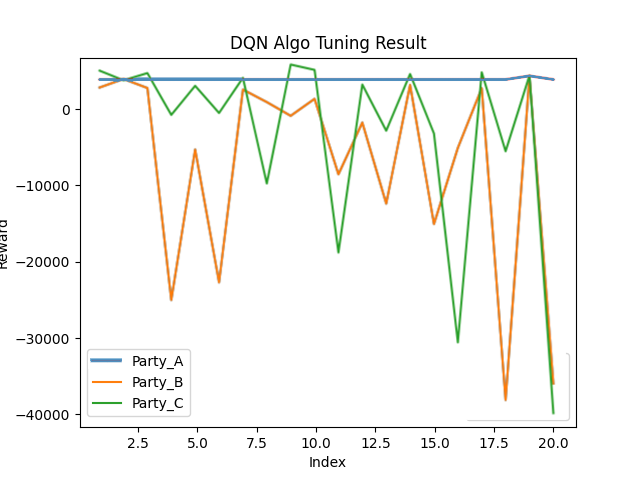
\includegraphics[width=\linewidth]{DQN.png}
    \caption{Result from DQN model}
    \label{fig:DQN}
\end{subfigure}
\begin{subfigure}{0.45\textwidth}
    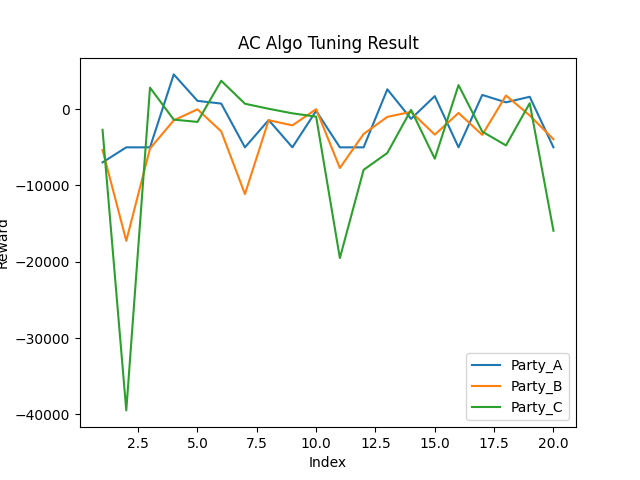
\includegraphics[width=\linewidth]{AC.png}
    \caption{Result from AC model}
    \label{fig:AC}
\end{subfigure}
\begin{subfigure}{0.45\textwidth}
    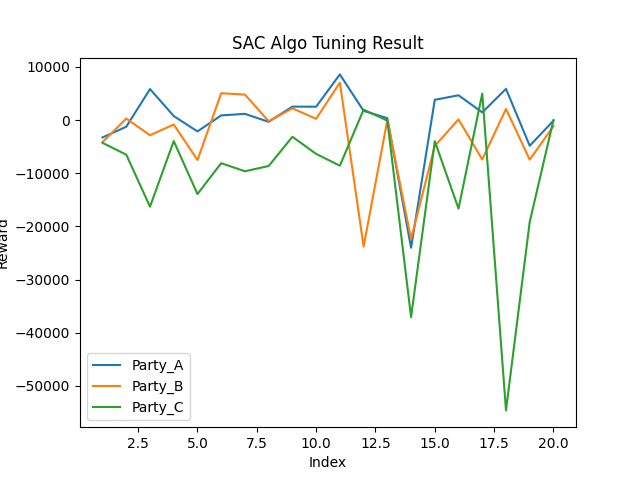
\includegraphics[width=\linewidth]{images/CAC.png}
    \caption{Result from CAC model}
    \label{fig:CAC}
\end{subfigure}
\caption{Reward curves from 20 test iterations}
\label{fig:select}
\end{figure}

The results from the mentioned test loops have been exhibited in the above Figure \ref{fig:select}:
\begin{itemize}
    \item The rewards from DQN model, as shown in Figure \ref{fig:DQN}, indicates its unsatisfying training within the designated time span, with significant fluctuation and predominant negative rewards.
    \item That provided by AC model, plotted in Figure \ref{fig:AC}, hints reduced uncertainty in rewards, despite of its high frequency of negative rewards and the lesser magnitude of positive rewards compared to its negative counterparts.
    \item The CAC model, as in Figure \ref{fig:CAC}, offers the best performance among all, evidenced by its increased level of positive rewards and reduced standard deviation.
\end{itemize}
Therefore, according to the outcomes from the aforementioned testing, CAC algorithm shows the best potential out of all, in regard to addressing this paper's problem. As a result, this model, Continuous Actor-Critic (CAC) algorithm will be implemented in the following numerical experiments.

To close this subsection, the reasons why the other two models underperformed are proposed. For both of DQN and AC, a discrete action space is required. However, in this paper's problem, an order can be precise up to the second decimal place. Despite the viability of dividing the action space onto a grid of 0.01, doing so significantly augments the dimension of Q matrix, leading to an soar in the dimensions. This impedes the efficiency of the training process. A workaround is to apply a less accurate discretisation in order for increased time-efficiency, but the actions are circumscribed to a compromised accuracy, resulting in poor performance;  Additionally, an intrinsic defect in DQN is that it needs a delicate hyperparameter tuning to handle the trade-off between exploration and exploitation, where an undershooting behaviour might arise.

\clearpage

\subsection{Analysis of the Selected Model}
In this subsection, the decided model, CAC, will be thoroughly trained and tested, upon which an assessment and analysis will be conducted. This will elucidate the impact of collusion, the reactions and countermeasures against market volatility, the situation where an enhanced stability is ensured by the collaboration.

To attain a promising set of parameters for the CAC neural networks, an intense training process has been conducted. Subject to the time costs and the limitation of computational power, an optimal result is not guaranteed. Instead, the optimised model is provided by the best outcome throughout an training of an acceptable amount of time.

In the first place, the optimised model is examined by a test consisting of 20 single iterations. The performance of the model is demonstrated in Figure \ref{fig:single}:
\begin{figure}[h]
    \centering
    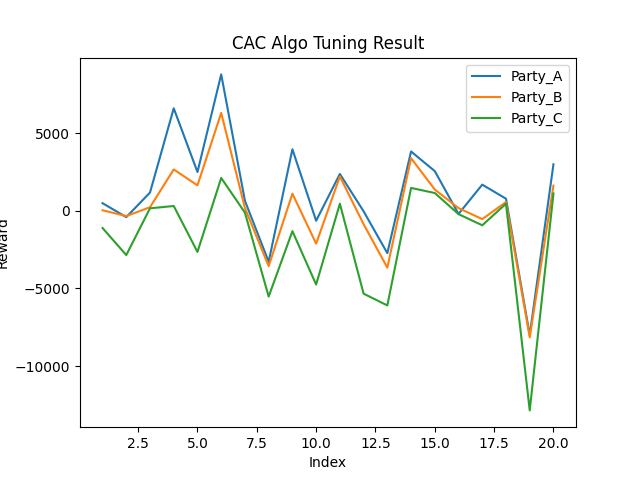
\includegraphics[scale=0.7]{images/CAC_2.png}
    \caption{The optimised result from CAC model: single iteration}
    \label{fig:single}
\end{figure}

Party A and Party B are able to gain positive rewards under most conditions, verifying the validity of this model and the effectiveness of the training. Party C's pronounced losses money notwithstanding, the downsized level of losses indicated an advancement from the previous model before optimisation. Plus, the underperfomance of Party C is foreseeable, since Party C's lack of intelligence has been configured by a limited neural network complexity. From an overarching perspective, the fluctuations in all of the parties seem to follow a similar pattern, a suggested explanation for which is all the traders are influenced by the volatility in the market. The edges between all the parties are not at a constant level, evidenced by the several intersections of curves and the huge gap seen at Iteration 4 and 5.


To analyse the behaviour of the model in a long and converged term, the optimised model is then attested through 15 rounds of 30 iterations apiece. The rewards in each round are the averaged and plotted in Figure \ref{fig:ave} below:
\begin{figure}[!ht]
    \centering
    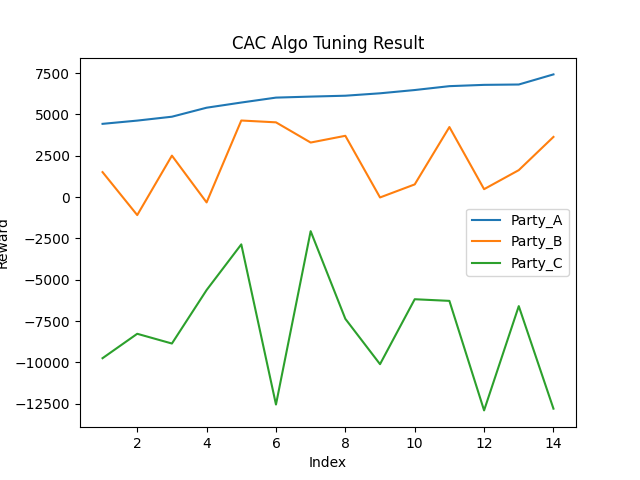
\includegraphics[scale=0.7]{images/Average.png}
    \caption{Average of 30 iterations (sorted by the values of party A)}
    \label{fig:ave}
\end{figure}

In a long run, the magnitude of each party's rewards is well-stratified, with no overlap spotted from the chart. Party A exhibits the most robust profitability, approximately 5,000 with minor undulation, Party B has obtained mostly positive rewards with moderate uncertainty and several outliers fallen under 0, while Party C has experienced substantial losses. Since Party A and Party B are set up with identical structures of their neural network and are trained through the same process, the only plausible reason for the discrepancy in rewards is that the collusion and reallocation of financial resources avail and enhance the profitability. Besides, the compromised performance of Party C implied that the existence of collusion sacrifices of the interest of less intelligent or less informed traders, potentially leading to inequality.

This analysis can also be corroborated by the statistics in Table \ref{tb:op-stats} in a more precise and quantified approach.

\begin{table}[!ht]
\centering
\caption{Statistics from the optimal model testing}
\label{tb:op-stats}
\begin{tabular}{|c|ccc|ccc|}
\hline
\cellcolor[HTML]{ECF4FF} & \multicolumn{3}{c|}{\textbf{Single Iteration}} & \multicolumn{3}{c|}{\textbf{30 Iterations}} \\ \cline{2-7} 
\cellcolor[HTML]{ECF4FF} & Party A       & Party B       & Party C        & Party A      & Party B      & Party C       \\ \hline
\textbf{Mean}            & 1153.25       & 111.92        & -1826.79       & 5987.16      & 2109.99      & -8014.73      \\
\textbf{STD}             & 3466.30       & 2915.62       & 3508.69        & 853.97       & 1869.93      & 3296.40       \\
\textbf{ARSD}            & 3.00          & 26.05         & 1.92           & 0.14         & 0.88         & 0.41          \\ \hline
\end{tabular}
\end{table}

Data in this table re-confirmed the above analysis: A bigger party in collusion outmanoeuvred the individual trader in party B, achieving a dominance with its increased profits, and the less intelligent trader in party C is disadvantaged in this market of imperfect competition. Additionally, the convergence of these identical independent experiments is verified by the dwindling STD and ARSD (Absolute Relative Standard Deviation).
\clearpage

\subsection{Sensitivity Test}
In this section, the initial configuration of the market and the learning agents is modified to investigate the robustness and effectiveness of our trained model, under the condition that an unexpected impact has been exerted on the system. Such an experiment is known as sensitivity test, as it aims to delve into how sensitive the model of concern is when it faces uncertainties.

The features that falls in the interest of this paper are: market volatility ($\sigma_0=1.00$), admissible inventory interval ($q_0\in[-20,20]$), market liquidity ($L^q_0=1\times 10^5$), buy and sell intensity ($BSI_0=10$), order volume multiplier ($M_0=10$) and initial fund of each agent ($F_0=5\times 10^5$). The initial values applied in previous training and testing are annotated in the brackets.

To evaluate the influence of fluctuations in each of these feature to the model's performance, one of them is selected and modified while the others are preserved, and then a 20 trading sessions are executed with the same model as before. The detail of the alteration is registered in Table \ref{tb:mod}.

\begin{table}[ht]
\caption{Detail of the modification}
\label{tb:mod}
\begin{tabular}{|c|cccccc|}
\hline
\textbf{Feature} & \textbf{Volatility} & \textbf{Inventory} & \textbf{Liquidity} & \textbf{BS Intensity} & \textbf{Multiplier} & \textbf{Fund} \\ \hline
\textbf{Original Val.} & 1 & 20 & 1e5 & 10 & 10 & 5e5 \\
\textbf{Modified Val.} & 2 & 10 & 1e3 & 5 & 3 & 1e4 \\
\textbf{Change (\%)} & 100\% & -50\% & -99\% & -50\% & -70\% & -98\% \\ \hline
\end{tabular}
\end{table}

Afterwards, the rewards from each session are recorded, plotted and labelled by its modified feature. Accordingly, a visualisation of such a sensitivity test is performed and displayed in Figure \ref{fig:ST}, whereas an essential statistical analysis is illustrated in Table \ref{tb:ST}. The change from each entry to its original counterpart is computed and displayed in percentage form, with the highlighted cells indicating an improved performance in the current entry. As a clarification, an improved performance are either an increased Max, Min or Mean, or a reduced STD or ARSD.



\begin{table}[ht]
\caption{Statistics from sensitivity test}
\label{tb:ST}
\begin{tabular}{|c|c|ccccc|ccccc|}
\hline
{\color[HTML]{333333} } & {\color[HTML]{333333} } & {\color[HTML]{333333} } & {\color[HTML]{333333} } & {\color[HTML]{333333} } & {\color[HTML]{333333} } & {\color[HTML]{333333} } & \multicolumn{5}{c|}{{\color[HTML]{333333} \textbf{Change (Percentage \%)}}} \\ \cline{8-12} 
\multirow{-2}{*}{{\color[HTML]{333333} \textbf{Mod.}}} & \multirow{-2}{*}{{\color[HTML]{333333} \textbf{P.}}} & \multirow{-2}{*}{{\color[HTML]{333333} \textbf{Max}}} & \multirow{-2}{*}{{\color[HTML]{333333} \textbf{Min}}} & \multirow{-2}{*}{{\color[HTML]{333333} \textbf{Mean}}} & \multirow{-2}{*}{{\color[HTML]{333333} \textbf{STD}}} & \multirow{-2}{*}{{\color[HTML]{333333} \textbf{ARSD}}} & {\color[HTML]{333333} \textbf{Max}} & {\color[HTML]{333333} \textbf{Min}} & {\color[HTML]{333333} \textbf{Mean}} & {\color[HTML]{333333} \textbf{STD}} & {\color[HTML]{333333} \textbf{ARSD}} \\ \hline
{\color[HTML]{333333} } & {\color[HTML]{333333} A} & {\color[HTML]{333333} 8787.1} & {\color[HTML]{333333} -8003.8} & {\color[HTML]{333333} 1153.3} & {\color[HTML]{333333} 3466.3} & {\color[HTML]{333333} 3.0} & \cellcolor[HTML]{ECF4FF}{\color[HTML]{333333} 0\%} & \cellcolor[HTML]{ECF4FF}{\color[HTML]{333333} 0\%} & \cellcolor[HTML]{ECF4FF}{\color[HTML]{333333} 0\%} & \cellcolor[HTML]{ECF4FF}{\color[HTML]{333333} 0\%} & \cellcolor[HTML]{ECF4FF}{\color[HTML]{333333} 0\%} \\
{\color[HTML]{333333} } & {\color[HTML]{333333} B} & {\color[HTML]{333333} 6305.5} & {\color[HTML]{333333} -8151.0} & {\color[HTML]{333333} 111.9} & {\color[HTML]{333333} 2915.6} & {\color[HTML]{333333} 26.1} & \cellcolor[HTML]{ECF4FF}{\color[HTML]{333333} 0\%} & \cellcolor[HTML]{ECF4FF}{\color[HTML]{333333} 0\%} & \cellcolor[HTML]{ECF4FF}{\color[HTML]{333333} 0\%} & \cellcolor[HTML]{ECF4FF}{\color[HTML]{333333} 0\%} & \cellcolor[HTML]{ECF4FF}{\color[HTML]{333333} 0\%} \\
\multirow{-3}{*}{{\color[HTML]{333333} \textbf{Ori.}}} & {\color[HTML]{333333} C} & {\color[HTML]{333333} 2115.4} & {\color[HTML]{333333} -12860.0} & {\color[HTML]{333333} -1826.8} & {\color[HTML]{333333} 3508.7} & {\color[HTML]{333333} 1.9} & \cellcolor[HTML]{ECF4FF}{\color[HTML]{333333} 0\%} & \cellcolor[HTML]{ECF4FF}{\color[HTML]{333333} 0\%} & \cellcolor[HTML]{ECF4FF}{\color[HTML]{333333} 0\%} & \cellcolor[HTML]{ECF4FF}{\color[HTML]{333333} 0\%} & \cellcolor[HTML]{ECF4FF}{\color[HTML]{333333} 0\%} \\ \hline
{\color[HTML]{333333} } & {\color[HTML]{333333} A} & {\color[HTML]{333333} 6689.7} & {\color[HTML]{333333} -9378.6} & {\color[HTML]{333333} -171.7} & {\color[HTML]{333333} 3445.8} & {\color[HTML]{333333} 20.1} & {\color[HTML]{333333} -24\%} & {\color[HTML]{333333} -17\%} & {\color[HTML]{333333} -115\%} & \cellcolor[HTML]{C6EFCE}{\color[HTML]{333333} -1\%} & {\color[HTML]{333333} 570\%} \\
{\color[HTML]{333333} } & {\color[HTML]{333333} B} & {\color[HTML]{333333} 7109.1} & {\color[HTML]{333333} -32127.7} & {\color[HTML]{333333} -1678.6} & {\color[HTML]{333333} 8178.0} & {\color[HTML]{333333} 4.9} & \cellcolor[HTML]{FFC7CE}{\color[HTML]{333333} 13\%} & {\color[HTML]{333333} -294\%} & {\color[HTML]{333333} -1600\%} & {\color[HTML]{333333} 180\%} & \cellcolor[HTML]{C6EFCE}{\color[HTML]{333333} -81\%} \\
\multirow{-3}{*}{{\color[HTML]{333333} \textbf{Vol.}}} & {\color[HTML]{333333} C} & {\color[HTML]{333333} 11184.5} & {\color[HTML]{333333} -20529.5} & {\color[HTML]{333333} -2236.4} & {\color[HTML]{333333} 6864.1} & {\color[HTML]{333333} 3.1} & \cellcolor[HTML]{FFC7CE}{\color[HTML]{333333} 429\%} & {\color[HTML]{333333} -60\%} & {\color[HTML]{333333} -22\%} & {\color[HTML]{333333} 96\%} & {\color[HTML]{333333} 63\%} \\ \hline
{\color[HTML]{333333} } & {\color[HTML]{333333} A} & {\color[HTML]{333333} 8503.2} & {\color[HTML]{333333} -13145.5} & {\color[HTML]{333333} -182.9} & {\color[HTML]{333333} 5632.8} & {\color[HTML]{333333} 30.8} & {\color[HTML]{333333} -3\%} & {\color[HTML]{333333} -64\%} & {\color[HTML]{333333} -116\%} & {\color[HTML]{333333} 63\%} & {\color[HTML]{333333} 927\%} \\
{\color[HTML]{333333} } & {\color[HTML]{333333} B} & {\color[HTML]{333333} 9784.8} & {\color[HTML]{333333} -39219.2} & {\color[HTML]{333333} 184.4} & {\color[HTML]{333333} 10567.4} & {\color[HTML]{333333} 57.3} & \cellcolor[HTML]{FFC7CE}{\color[HTML]{333333} 55\%} & {\color[HTML]{333333} -381\%} & \cellcolor[HTML]{FFC7CE}{\color[HTML]{333333} 65\%} & {\color[HTML]{333333} 262\%} & {\color[HTML]{333333} 120\%} \\
\multirow{-3}{*}{{\color[HTML]{333333} \textbf{Inv.}}} & {\color[HTML]{333333} C} & {\color[HTML]{333333} 7155.7} & {\color[HTML]{333333} -28554.7} & {\color[HTML]{333333} -9788.8} & {\color[HTML]{333333} 9649.4} & {\color[HTML]{333333} 1.0} & \cellcolor[HTML]{FFC7CE}{\color[HTML]{333333} 238\%} & {\color[HTML]{333333} -122\%} & {\color[HTML]{333333} -436\%} & {\color[HTML]{333333} 175\%} & \cellcolor[HTML]{C6EFCE}{\color[HTML]{333333} -47\%} \\ \hline
{\color[HTML]{333333} } & {\color[HTML]{333333} A} & {\color[HTML]{333333} 670.0} & {\color[HTML]{333333} -1033.3} & {\color[HTML]{333333} -71.9} & {\color[HTML]{333333} 336.5} & {\color[HTML]{333333} 4.7} & {\color[HTML]{333333} -92\%} & \cellcolor[HTML]{FFC7CE}{\color[HTML]{333333} 87\%} & {\color[HTML]{333333} -106\%} & \cellcolor[HTML]{C6EFCE}{\color[HTML]{333333} -90\%} & {\color[HTML]{333333} 57\%} \\
{\color[HTML]{333333} } & {\color[HTML]{333333} B} & {\color[HTML]{333333} 1301.8} & {\color[HTML]{333333} -1180.5} & {\color[HTML]{333333} 56.4} & {\color[HTML]{333333} 447.5} & {\color[HTML]{333333} 8.8} & {\color[HTML]{333333} -79\%} & \cellcolor[HTML]{FFC7CE}{\color[HTML]{333333} 86\%} & {\color[HTML]{333333} -50\%} & \cellcolor[HTML]{C6EFCE}{\color[HTML]{333333} -85\%} & \cellcolor[HTML]{C6EFCE}{\color[HTML]{333333} -66\%} \\
\multirow{-3}{*}{{\color[HTML]{333333} \textbf{Liq.}}} & {\color[HTML]{333333} C} & {\color[HTML]{333333} 1340.5} & {\color[HTML]{333333} -1294.5} & {\color[HTML]{333333} -50.7} & {\color[HTML]{333333} 541.6} & {\color[HTML]{333333} 9.6} & {\color[HTML]{333333} -37\%} & \cellcolor[HTML]{FFC7CE}{\color[HTML]{333333} 90\%} & \cellcolor[HTML]{FFC7CE}{\color[HTML]{333333} 97\%} & \cellcolor[HTML]{C6EFCE}{\color[HTML]{333333} -85\%} & {\color[HTML]{333333} 405\%} \\ \hline
{\color[HTML]{333333} } & {\color[HTML]{333333} A} & {\color[HTML]{333333} 17579.6} & {\color[HTML]{333333} -21840.3} & {\color[HTML]{333333} -900.2} & {\color[HTML]{333333} 7473.0} & {\color[HTML]{333333} 8.3} & \cellcolor[HTML]{FFC7CE}{\color[HTML]{333333} 100\%} & {\color[HTML]{333333} -173\%} & {\color[HTML]{333333} -178\%} & {\color[HTML]{333333} 116\%} & {\color[HTML]{333333} 177\%} \\
{\color[HTML]{333333} } & {\color[HTML]{333333} B} & {\color[HTML]{333333} 5101.7} & {\color[HTML]{333333} -36839.2} & {\color[HTML]{333333} -4867.9} & {\color[HTML]{333333} 9454.9} & {\color[HTML]{333333} 1.9} & {\color[HTML]{333333} -19\%} & {\color[HTML]{333333} -352\%} & {\color[HTML]{333333} -4450\%} & {\color[HTML]{333333} 224\%} & \cellcolor[HTML]{C6EFCE}{\color[HTML]{333333} -93\%} \\
\multirow{-3}{*}{{\color[HTML]{333333} \textbf{BSI}}} & {\color[HTML]{333333} C} & {\color[HTML]{333333} 0.0} & {\color[HTML]{333333} -89456.0} & {\color[HTML]{333333} -20692.5} & {\color[HTML]{333333} 26146.9} & {\color[HTML]{333333} 1.3} & {\color[HTML]{333333} -100\%} & {\color[HTML]{333333} -596\%} & {\color[HTML]{333333} -1033\%} & {\color[HTML]{333333} 645\%} & \cellcolor[HTML]{C6EFCE}{\color[HTML]{333333} -32\%} \\ \hline
{\color[HTML]{333333} } & {\color[HTML]{333333} A} & {\color[HTML]{333333} 3893.1} & {\color[HTML]{333333} -1814.3} & {\color[HTML]{333333} 1145.1} & {\color[HTML]{333333} 1634.6} & {\color[HTML]{333333} 1.4} & {\color[HTML]{333333} -56\%} & \cellcolor[HTML]{FFC7CE}{\color[HTML]{333333} 77\%} & {\color[HTML]{333333} -1\%} & \cellcolor[HTML]{C6EFCE}{\color[HTML]{333333} -53\%} & \cellcolor[HTML]{C6EFCE}{\color[HTML]{333333} -53\%} \\
{\color[HTML]{333333} } & {\color[HTML]{333333} B} & {\color[HTML]{333333} 4575.5} & {\color[HTML]{333333} -6909.5} & {\color[HTML]{333333} -904.2} & {\color[HTML]{333333} 2857.7} & {\color[HTML]{333333} 3.2} & {\color[HTML]{333333} -27\%} & \cellcolor[HTML]{FFC7CE}{\color[HTML]{333333} 15\%} & {\color[HTML]{333333} -908\%} & \cellcolor[HTML]{C6EFCE}{\color[HTML]{333333} -2\%} & \cellcolor[HTML]{C6EFCE}{\color[HTML]{333333} -88\%} \\
\multirow{-3}{*}{{\color[HTML]{333333} \textbf{Mul.}}} & {\color[HTML]{333333} C} & {\color[HTML]{333333} -67.1} & {\color[HTML]{333333} -24531.2} & {\color[HTML]{333333} -4853.7} & {\color[HTML]{333333} 5595.3} & {\color[HTML]{333333} 1.2} & {\color[HTML]{333333} -103\%} & {\color[HTML]{333333} -91\%} & {\color[HTML]{333333} -166\%} & {\color[HTML]{333333} 59\%} & \cellcolor[HTML]{C6EFCE}{\color[HTML]{333333} -37\%} \\ \hline
{\color[HTML]{333333} } & {\color[HTML]{333333} A} & {\color[HTML]{333333} 7986.4} & {\color[HTML]{333333} -10000.0} & {\color[HTML]{333333} -2547.8} & {\color[HTML]{333333} 5314.9} & {\color[HTML]{333333} 2.1} & {\color[HTML]{333333} -9\%} & {\color[HTML]{333333} -25\%} & {\color[HTML]{333333} -321\%} & {\color[HTML]{333333} 53\%} & \cellcolor[HTML]{C6EFCE}{\color[HTML]{333333} -30\%} \\
{\color[HTML]{333333} } & {\color[HTML]{333333} B} & {\color[HTML]{333333} 11108.3} & {\color[HTML]{333333} -10000.0} & {\color[HTML]{333333} -4333.0} & {\color[HTML]{333333} 6369.0} & {\color[HTML]{333333} 1.5} & \cellcolor[HTML]{FFC7CE}{\color[HTML]{333333} 76\%} & {\color[HTML]{333333} -23\%} & {\color[HTML]{333333} -3972\%} & {\color[HTML]{333333} 118\%} & \cellcolor[HTML]{C6EFCE}{\color[HTML]{333333} -94\%} \\
\multirow{-3}{*}{{\color[HTML]{333333} \textbf{Fund}}} & {\color[HTML]{333333} C} & {\color[HTML]{333333} 5296.9} & {\color[HTML]{333333} -10000.0} & {\color[HTML]{333333} -6355.9} & {\color[HTML]{333333} 5103.6} & {\color[HTML]{333333} 0.8} & \cellcolor[HTML]{FFC7CE}{\color[HTML]{333333} 150\%} & \cellcolor[HTML]{FFC7CE}{\color[HTML]{333333} 22\%} & {\color[HTML]{333333} -248\%} & {\color[HTML]{333333} 45\%} & \cellcolor[HTML]{C6EFCE}{\color[HTML]{333333} -58\%} \\ \hline
\end{tabular}
\end{table}

\begin{figure}[ht]
\centering
\begin{subfigure}{0.95\textwidth}
    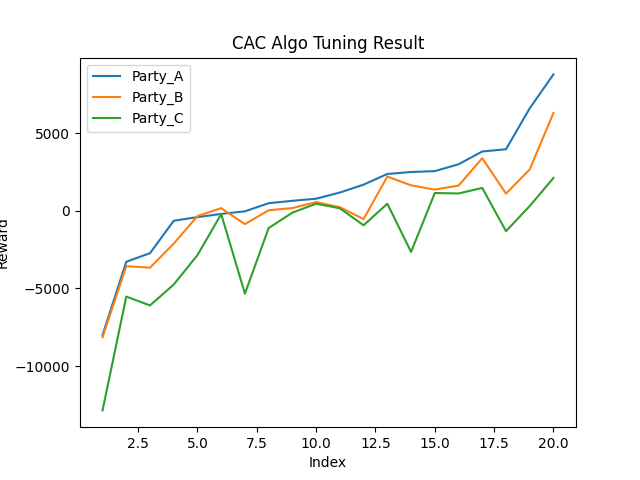
\includegraphics[width=0.48\linewidth]{images/single.png}
    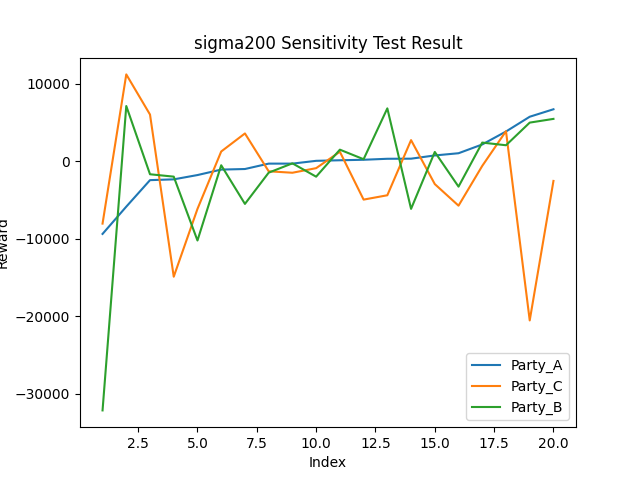
\includegraphics[width=0.48\linewidth]{images/ST_sigma200.png}
    \caption{Original data as in Figure \ref{fig:single} (left), doubled market volatility (right)}
    \label{fig:Ori&Vol}
\end{subfigure}

\begin{subfigure}{0.95\textwidth}
    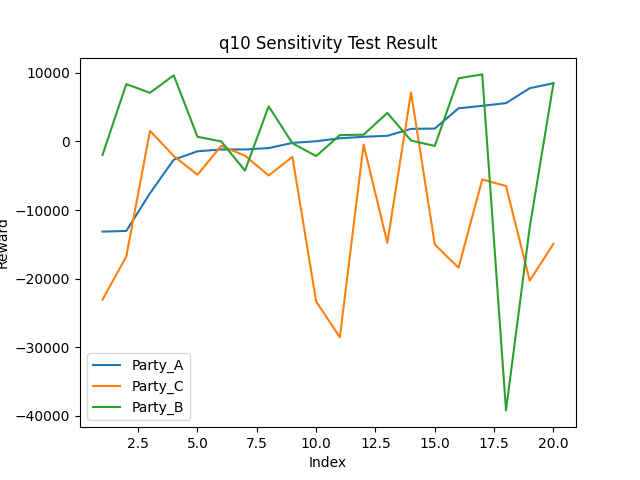
\includegraphics[width=0.48\linewidth]{images/ST_q10.png}
    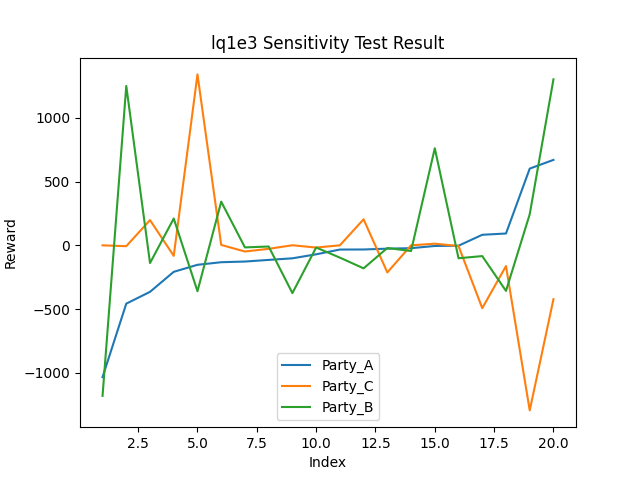
\includegraphics[width=0.48\linewidth]{images/ST_lq1e3.png}
    \caption{Halved admissible inventory (left), 1.00\% market liquidity (right)}
    \label{fig:Inv&Liq}    
\end{subfigure}

\begin{subfigure}{0.95\textwidth}
    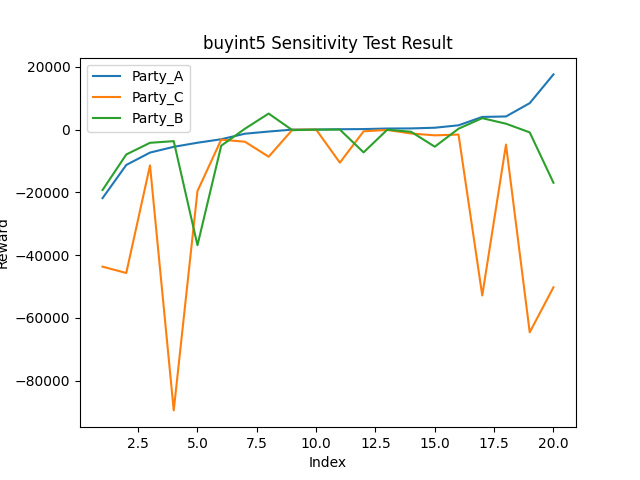
\includegraphics[width=0.48\linewidth]{images/ST_buyint5.png}
    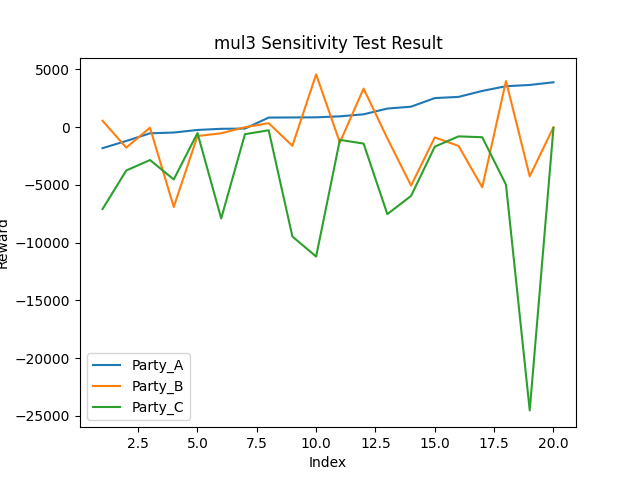
\includegraphics[width=0.48\linewidth]{images/ST_mul3.png}
    \caption{Halved buy and sell intensity (left), 30\% order volume multiplier (right)}
    \label{fig:BSI&Mul}
\end{subfigure}

\begin{subfigure}{0.45\textwidth}
    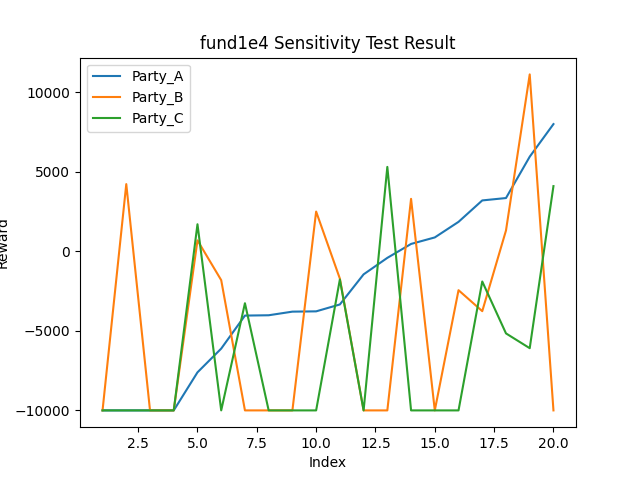
\includegraphics[width=\linewidth]{images/ST_fund1e4.png}
    \caption{2\% initial fund}
    \label{fig:Fund}
\end{subfigure}

\caption{Reward curves from sensitivity test}
\label{fig:ST}
\end{figure}


In a panoramic view, in a modified market environment, the profitability of the colluded traders and the intelligent trader has been seen waning, as confirmed by the mostly dipped mean rewards. The excessive profit of the colluded party is also impaired, since an increased number of intersections occurred between Party A's reward curves and others', which, in other words, implies that Party A is frequently outplayed by other parties without collusion. Although in general, a plunge of profits strikes to each party, in some scenarios, as a result of Party A and B's weakened market positions, Party C's profits roared, as can be spotted in the bottom row of in Li1. section. 

However, an advantage the cartel has during such impacts is its stability. As shown in the STD column of Table \ref{tb:ST}, the absolute STD (on the contrary to the relative STD) of Party A is almost always the lowest among all, which is also evidenced by its less drastic fluctuations seen in Figure \ref{fig:ST}. Besides, the changes occurred to Party A are almost always the most favourable among all there parties, reaffirming its immunity against market uncertainty.

In brief, with an impact from the market environment, the excessive profitability of the intelligent trader and the cartel is contained, whereas the less intelligent agent occasionally shows an advanced performance. The weakened dominance nonetheless, the existence of collusion buttresses the cartel's stability.

To probe into a microscopic layer and explain its counteractions, an elaborate analysis of the model's response to each feature is provided:
\begin{itemize}
    \item Market volatility: An doubled market volatility might lead to the failure of a trained model to capture the actual optimal decision, since adopting a progressive manner of trading may result in great loss and vice versa. As expected, this causes significant drop in Party A and B's profit, in contrast to the moderate level of losses happened to Party C. However, the collusion inoculated the cartel against this upturned volatility through the re-allocation of resources, facilitating a reduced STD.
    \item Admissible inventory interval: An halved admissible inventory interval tightens the inventory one can possesses. This would help a trader if they could not formulate an effective risk-mitigating strategy. Since Party B's rewards are reinforced, its trading strategies are presumably more aggressive, which such a downturned interval helps to offset. 
    \item Market liquidity: A limited market liquidity slows tradings down, as there might not be an liquidated asset that meets the requirements of an order in the market, so the order will have to stay pending until such an asset is provided and released. As a consequence, an enhanced stability stems from the slowdowns, instantiated by the shrunken STD, and the Min values, namely, the most drastic losses in this case, experience a surge, supposedly because a slower trading process ameliorates the effects of risk. The lessened risk aside, Party A and B undershoot compared to the original case, since the limitation on liquidity enacts a barrier for trades, which, however, remedies Party C from its disadvantaged market position, evidenced by its increased mean of rewards.
    \item Buy and sell intensity: Buy and sell intensity determines the frequency of orders emerging on the market. Therefore, a halved buy and sell intensity has an material influence on the optimal trading strategies, as it approximately reduces the amount of orders on the market, resulting in accrued orders that could have been agreed under the original market setting. This effect significantly nullifies the model and engenders fierce losses as can be spotted in the mean rewards.
    \item Order volume multiplier: A scaled-down volume multiplier will pass the same scaling effect directly onto the order's volume. Thus, it almost scales losses and gains by the same intensity. Since the mean rewards of Party A and B are mostly positive, it overall slashes the level of gains, leading to a less ideal performance. The opposite is true for Party C. The different patterns in STD also proves that the colluded party has the best robustness, whereas the less intelligent trader might be involved in and impacted by the market configuration to a greater extent.
    \item Initial fund: The initial fund not only determines the scope of financial resources one commands, but also affects the replenishment of the margin account. While it controls the loss within the initial fund — namely, one cannot lose more than one used to have— it increases the probability of a closed out position. Consequently, lessened levels of Min-reward of Party C are witnessed, since the losses are more tightly lower-bounded and this mechanism is more critical for traders in weaker positions. Despite this automated risk-management function, the lack of capital leads to more conspicuous underperformance of the dominant parties than Party C, since trading with their previous aggressive manner requires adequate financial resources, that are not granted in this limited initial fund setting.
\end{itemize}
\clearpage





\section{Conclusions}
In this study, the mathematical framework of reinforcement learning has been introduced, and by the assurance of the theorems behind, three different algorithms, DQN, AC and CAC, have been proposed for training automated traders in the futures market set in Vega's platform. Throughout a test of each algorithm, the model underpinned by CAC exhibits the most ideal performance out of all, and therefore it has been selected for the numerical practice in this paper, where four traders are divided into three parties with the first one forming a cartel with collusion and an equal asset reallocation, the second one of a tantamount intelligence level and the third one of limited intelligence, as a emulation for a less informed and professional trader in the market.

The optimised CAC model (best performance among results obtained in limited training time) indicates a satisfying profitability for all intelligent parties and a tendency of convergence, having verified the validity of the chosen model. In details of each party, there is an edge of the cartel's profits over the individual intelligent trader, a indicator of the enhanced margin accomplished with the assistance of collusion. A sacrificed profitability has been observed in the third party, a testament of the intelligent traders' dominance and the disadvantage an "amateur" trader might be at in this risk-intense futures market.

Albeit the promising performance, the robustness of this model is problematic in a minor way, discovered during the sensitivity test. Upon any changes to the market configuration, the rewards provided by the model fail to show enough resistance to uncertainties, and negative mean rewards have been spotted in a majority of the cases. However, a comparatively better immunity against changes has been perceived in the cartel, substantiating that the collusion mitigates the market risk.

Throughout this research, measures that might improve the model's behaviour and subjects that have not been investigated have come to light. These findings lay the foundation of the recommendations for further development:
\begin{itemize}
    \item The training process is circumscribed by the hardware and the limited time, so a more thorough training might be needed to achieve an improved performance.
    \item The robustness examined by the sensitivity test is still sub-optimal, and therefore there is room for future refinement. A different model or an pre-training based on historical data to glean information from the market may advance the performance.
    \item The code configures the setting of agents and the parties they belong to in a flexible manner, and hence various scenarios can be put into tests without much further ado. An increased size of the cartel, different level of intelligence and an greater number of individual traders may have substantial influence on the model's behaviour, and the associated topics might proffer insightful discoveries.
    \item A perfectly competitive condition can be simulated in a market of all individual traders, the result of which can be used as a benchmark to precisely gauge the actual level of excessive profit coinciding with the existence of collusion.
\end{itemize}



\clearpage

%the entries have to be in the file literature.bib
\bibliography{literature}
\clearpage

\appendix
\section*{Appendices}
\addcontentsline{toc}{section}{Appendices}

\section{Source Code}
For inspection, future refinement and collaboration, the source code that has been used throughout this study is uploaded to the following GitHub link: https://github.com/RoyceYan/vega-market-sim. This is forked from the original open source repository, added with the the code this paper applied. To trace the commits made for this specific study, navigate to the MSc branch and look for commits by RoyceYan.
\clearpage

\end{document}